%%=============================================================================
%% Methodologie
%%=============================================================================

\chapter{\IfLanguageName{dutch}{Methodologie}{Methodology}}%
\label{ch:methodologie}

%% TODO: In dit hoofstuk geef je een korte toelichting over hoe je te werk bent
%% gegaan. Verdeel je onderzoek in grote fasen, en licht in elke fase toe wat
%% de doelstelling was, welke deliverables daar uit gekomen zijn, en welke
%% onderzoeksmethoden je daarbij toegepast hebt. Verantwoord waarom je
%% op deze manier te werk gegaan bent.
%% 
%% Voorbeelden van zulke fasen zijn: literatuurstudie, opstellen van een
%% requirements-analyse, opstellen long-list (bij vergelijkende studie),
%% selectie van geschikte tools (bij vergelijkende studie, "short-list"),
%% opzetten testopstelling/PoC, uitvoeren testen en verzamelen
%% van resultaten, analyse van resultaten, ...
%%
%% !!!!! LET OP !!!!!
%%
%% Het is uitdrukkelijk NIET de bedoeling dat je het grootste deel van de corpus
%% van je bachelorproef in dit hoofstuk verwerkt! Dit hoofdstuk is eerder een
%% kort overzicht van je plan van aanpak.
%%
%% Maak voor elke fase (behalve het literatuuronderzoek) een NIEUW HOOFDSTUK aan
%% en geef het een gepaste titel.

% \lipsum[21-25]

Het doel van dit onderzoek is het ontwikkelen van een machine learning-pijplijn die effectief veranderingen 
kan detecteren tussen de aanwezigheid van vegetatie tussen twee tijdstippen. Dit is een vergelijkende studie, 
waarbij verschillende machine learning modellen getraind en geëvalueerd worden.
\newline
\section{\IfLanguageName{dutch}{Image preprocessing}{Image preprocessing}}%
\label{sec:image-preprocessing}
De eerste fase van het onderzoek is het samenstellen van twee datasets opgebouwd uit luchtfoto's van Geopunt Vlaanderen. De afbeelding hebben
het jpeg 2000 formaat. De training dataset bestaat uit afbeeldingen van verschillende Vlaamse steden tussen 2020 (t₁) en 2024 (t₂). 
Tijdens de trainingsfase wordt deze dataset gebruikt om het model te leren veranderingen in vegetatie te ontdekken tussen de twee tijdstippen.
De test dataset bestaat uit afbeeldingen van Gent tussen 2020 (t₁) in 2024 (t₂). Deze dataset wordt gebruikt voor model evaluatie.
\newline
Data wordt ingeladen met rasterio, een python library voor het gebruiken van GIS data. De afbeeldingen worden herschaalt naar (2560, 2560, 3).
Hierna wordt de foto opgedeeld in 100 (256, 256, 3) patches. De foto's worden gelabeld met behulp van de excess green index (ExG).
Deze index maakt gebruik van de rgb waarden van een afbeelding om vegetatie automatisch te laten generen: \(ExG = 2 * Green - Red - Blue \).
% het QUPath programma. In beide foto's wordt de vegetatie aangeduid. 
Hieruit ontstaan twee distincte vegetatie masks. Door de mask van (t₂) wiskundig te verminderen met die van (t₁) 
bereken we change labels tussen beide afbeeldingen. De training data wordt opgeslagen in een python lijst bestaande uit tuples van 
voor en na afbeeldingen (ndarray's). De lijst heeft een lengte van 600. 
% De test data (afbeeldingen van Gent) bestaat 100 tupels van afbeeldingen.
\newline
\section{\IfLanguageName{dutch}{CGNet}{CGNet}}%
\label{sec:cgnet}
Change guidding network (CGNet) is een convolutional neuraal netwerk voorgesteld in de studie van \textcite{Han2023}. 
Een model ontworpen voor change detection als reactie op de tekortkomingen van de UNet architectuur in verband met edge detection en 
internal holes.
\newline
\newline
\begin{figure*}
  \centering
  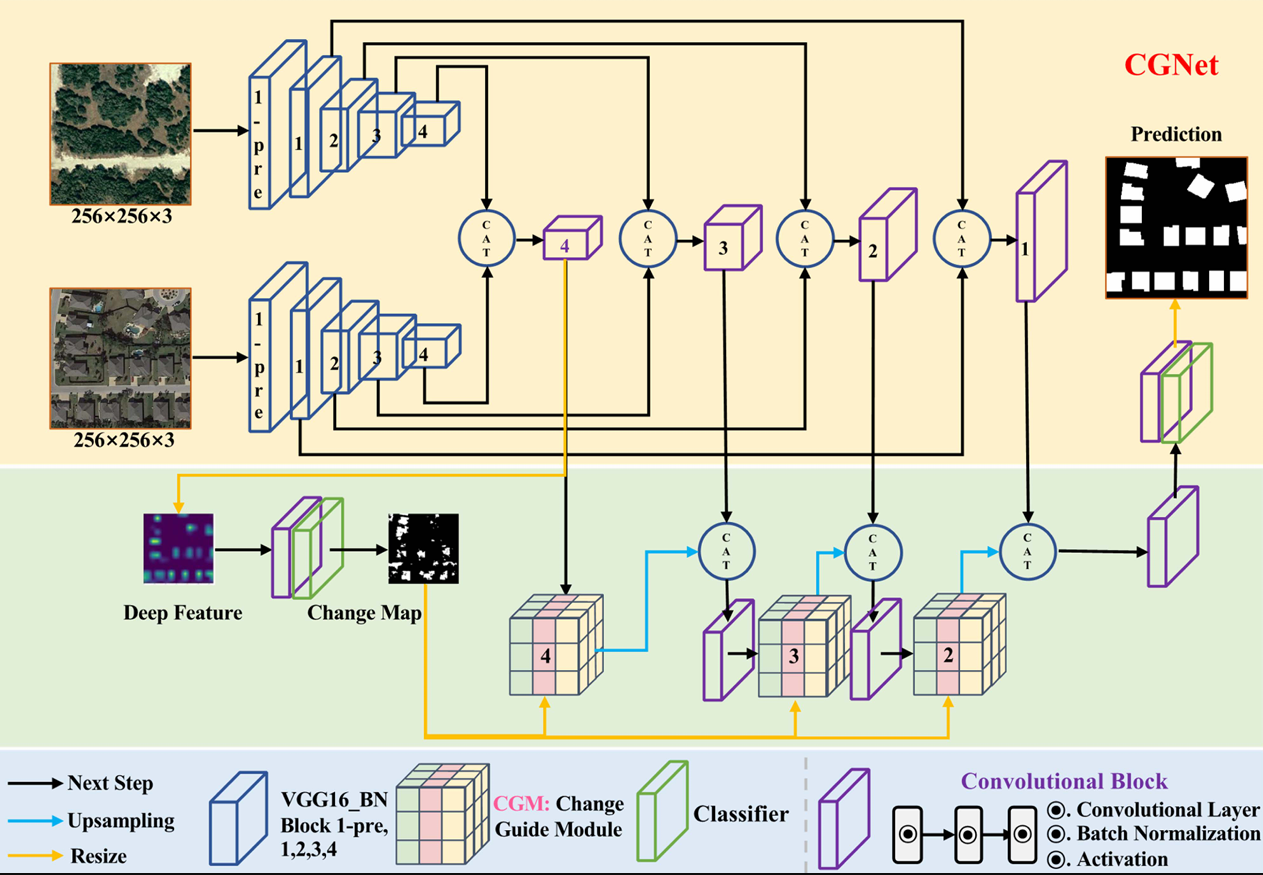
\includegraphics[width=\textwidth]{CGNet.png}
  \caption{\label{fig:CGNet}CGNet architectuur \autocite{Han2023}.}
\end{figure*}
Het model is opgedeeld in drie delen. Een encoder bestaande uit vijf VGG-16 blocks gevolgd door batch normalisatie. De decoder waar 
feature extractie wordt toegepast. Features van de encoder worden toegepast op een convolutional blocks opgemaakt uit een convolutional
layer, batch normalisatie en de ReLU activatie functie. De change map ontstaat door deep features, output van de eerste convolutional block
van de decoder, door een convolutional block gevolgd door een classificatie layer te sturen. De change guide module (CGM) is een self-attention 
architectuur voor het identificeren van de features die veranderingen tussen de twee afbeeldingen tonen. Deze features worden doorgeven, 
terwijl de andere worden gedropt. De output van de CGM's en de decoder worden samengevoegd en na twee convolutional blocks 
geclassificeerd in een change map als output van het model.
\newline
\newline
De pythorch library wordt gebruikt om de data klaar te maken voor het model. De dataset class transformeert de foto's van ndarray's naar 
pythorch tensors. De pythorch dataloader class biedt een itereerbare methode over de gegeven dataset. De batch size van de dataloader is vier en
de shuffle optie staat aan.
\newline
\newline
Tijdens de model training wordt de BCE With Logits Loss gebruikt. Deze loss functie 
combineert een sigmoïd functie en de BCELoss functie in één enkele klasse. Deze versie is numeriek stabieler dan een gewone Sigmoïd functie. 
De formule van de loss functie: \(l(x,y) = L = \{l_1,\ldots,l_N\}^T \), \(l_n = -w_n[y_n * \log\sigma(x_n) + (1-y_n) * 
\log(1 - \sigma(x_n))] \), waar N de batch size is.
\newline
\newline
Als optimizer gebruiken we adam. De Adaptive Moment Estimation combineert de voordelen van Momentum- en RMSprop-technieken om de 
leersnelheid tijdens de training aan te passen. Het werkt goed met grote datasets en complexe modellen omdat het geheugen efficiënt 
wordt gebruikt en de leersnelheid voor elke parameter automatisch wordt aangepast. Het model wordt getraind voor 10 epochs.

\section{\IfLanguageName{dutch}{ChangeFormer}{ChangeFormer}}%
\label{sec:change-former}
Changeformer is een siamese transformer neuraal netwerk voor change detection geïntroduceerd in het onderzoek van \textcite{Bandara2022}.
Het netwerk bestaat uit twee siamese twin transformer encoders, opgebouwd uit transformer en downsampeling blocks. Downsampeling van de input 
gebeurt initieel met een convolutional layer met Kernel=3, Stride=2 en Padding=1. De eerste downsampeling block heeft een convolutional layer 
met Kernel=7, Stride=4 en Padding=3. Na een downsampeling block volgt altijd een een transformer block. Dit is een 
self-attention layer met als doel de complexiteit van de input te verminderen door alleen de belangrijkste features te behouden. 
Er zijn vier difference modules die aan de hand van de features van de encoder veranderingen tussen de twee inputs berekenen. Het bestaat
uit batch normalisatie en een convolutionele layer gevolgd door de ReLU activatie functie. De weights van beide encoders worden met elkaar gedeeld.
\newline
\newline
\begin{figure*}
  \centering
  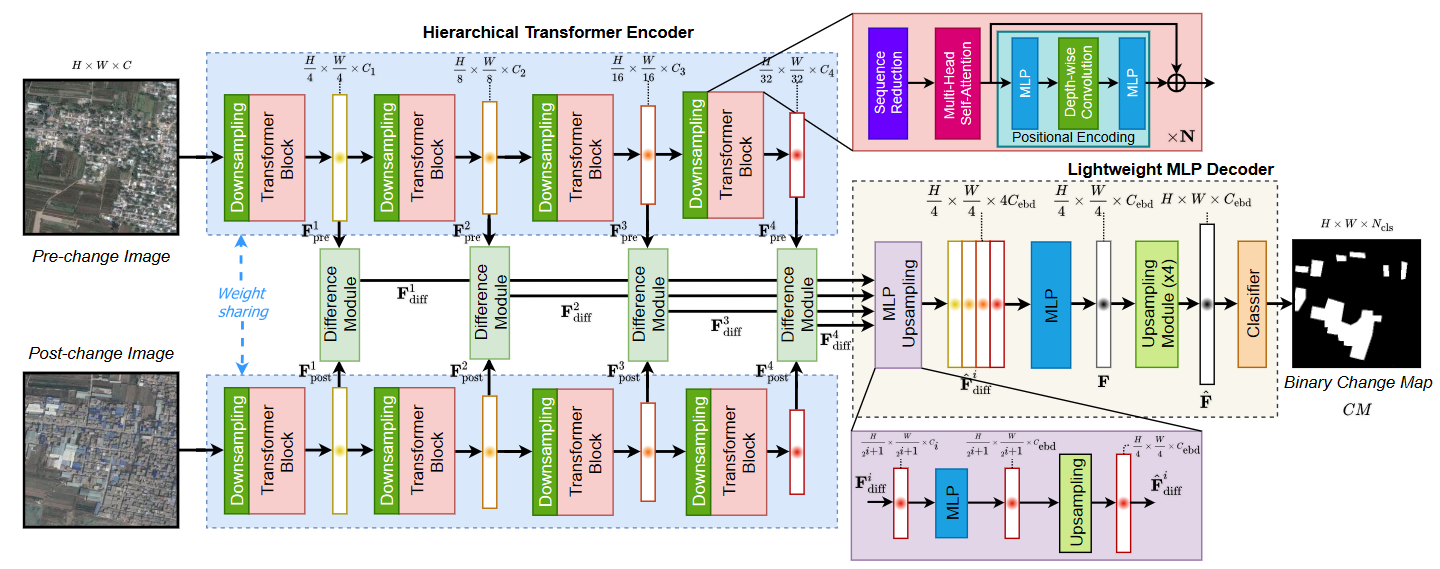
\includegraphics[width=\textwidth]{ChangeFormer.png}
  \caption{\label{fig:CF}ChangeFormer architectuur \autocite{Bandara2022}.}
\end{figure*}
De MLP decoder gebruikt de output van de finale difference module (vier feature difference maps) om zo de change map te voorspellen.
Eerst is er een MLP layer gevolgd door een upsampling layer die de feature difference maps herschalen naar de originele afmeting van de input. 
Hierna worden alle feature maps samengevoegd met behulp van een MLP layer. Met nog een upsampling layer en tenslotte een classificatie MLP layer. 
\newline
\newline
De data wordt ge preprocessed door de dataset en dataloader pythorch classes. De foto's worden omgezet in pythorch tensors. De loader heeft een
batch size = 4. Het model is gedeclareerd met de decoder softmax optie op false. Dit komt omdat we binaire en geen multi-label classificatie doen.
Als loss functie gebruiken we de Cross Entropy Loss. Dit criterium berekent het cross entropy loss tussen input logits en target values.
Het model gebruikt de adam optimizer. De data wordt getraind in 10 epochs.
\newline
\newline

\section{\IfLanguageName{dutch}{Random Forest}{Random Forest}}%
\label{sec:random-forest}
Voor dit deel van het onderzoek wordt de RandomForestClassifier class van de sklearn library gebruikt. Eerst reshapen we de training data 
naar een 2D array waarin elke rij een pixel voorstelt. Vervolgens wordt de data van (t₁) en (t₂) gecombineerd tot één feature. 
De change masks (labels) worden omgezet naar een 1D-array. Het model wordt geïnitialiseerd met 100 decision trees (n estimators). 
Dan start het trainingsproces. Elke paar afbeeldingen wordt apart getraind.
\newline
\newline

\section{\IfLanguageName{dutch}{SVM}{SVM}}%
\label{sec:svm}
Het Support vector machine model dat gebruikt wordt is afkomstig van de sklearn library. De features worden handmatig berekent. 
We reshapen de features naar een 2D-array waarbij elke pixel een rij is. De labels worden omgezet naar een 1D-array. Voor het model gebruiken we 
de rfb kernel en zetten probability op false. Dit doen we om het trainingsproces te versnellen. Het model wordt apart getraind op elk foto paar.
\newline
\newline

% Het doel van dit onderzoek is de ontwikkeling van een machine learning-pijplijn die op een efficiënte en nauwkeurige wijze veranderingen 
% in vegetatiebedekking kan detecteren tussen twee verschillende tijdstippen. Dit onderzoek omvat een vergelijkende studie waarbij 
% verschillende machine learning-modellen worden geëvalueerd op hun effectiviteit in change detection.
% \newline
% \newline
% De eerste stap in de methodologie betreft de constructie van twee datasets bestaande uit luchtfoto's genomen door het agentschap 
% digitaal Vlaanderen (middenschalige orthofotobedekking van het Vlaamse Gewest). De eerste dataset bevat afbeeldingen van de stad Gent 
% uit 2020 (t₁), terwijl de tweede dataset bestaat uit beelden van Gent uit 2024 (t₂). De analyse wordt uitgevoerd door de beelden 
% van t₁ en t₂ met behulp van machine learning-methoden te vergelijken om vegetatieveranderingen te identificeren.
% \newline
% \newline
% De datasets worden onderverdeeld in drie segmenten: training (60\%), validatie (20\%) en testing (20\%). 
% De trainingsfase dient om het model te optimaliseren op basis van gelabelde data, terwijl de validatiefase wordt gebruikt om de prestaties 
% van het model te evalueren op niet eerder geziene gegevens, waardoor overfitting wordt geminimaliseerd. 
% De testfase wordt vervolgens ingezet om de uiteindelijke modelprestaties te beoordelen. Een representatieve dataset is hierbij 
% essentieel om de generaliseerbaarheid van het model te waarborgen, zodat seizoensgebonden variaties en andere omgevingsfactoren correct 
% worden verwerkt.
% \newline
% \newline
% Vooraf gedefinieerde machine learning-modellen worden getraind en getest op de dataset, waarbij gebruik wordt gemaakt van 
% pretrained modellen in plaats van een model vanaf nul op te bouwen. De dataset wordt vooraf verwerkt via een preprocessing-stap, 
% waarbij technieken zoals rescaling (data-augmentatie) worden toegepast om alle afbeeldingen naar een uniforme resolutie te schalen. 
% De data wordt geannoteerd via semantische segmentatie, een computer vision-techniek waarbij elke pixel wordt toegewezen aan een specifieke 
% klasse (bijvoorbeeld vegetatie, gebouwen of wegen). Dit resulteert in een segmentatiekaart die een gedetailleerd overzicht biedt van de 
% objecten binnen de afbeelding.
% \newline
% \newline
% Om veranderingen tussen t₁ en t₂ te detecteren, worden verschillen in kenmerken zoals gemiddelde kleur, objectgrootte en vormvariatie 
% geanalyseerd. Vervolgens worden deze veranderingen geclassificeerd, waarbij niet alleen de aanwezigheid van verandering wordt vastgesteld, 
% maar ook de aard van de transformatie binnen de objecten.
% \newline
% \newline
% Voor de evaluatie van de verschillende machine learning-modellen worden meerdere prestatie-indicatoren gehanteerd. 
% De Vegetation Condition Index (VCI) wordt als primaire metriek gebruikt om veranderingen in vegetatiebedekking te kwantificeren door 
% de Normalized Difference Vegetation Index (NDVI)-waarden van t₁ en t₂ met elkaar te vergelijken. Daarnaast worden aanvullende 
% evaluatiemethoden toegepast, waaronder confusion matrix-gebaseerde metrieken zoals precision en recall, evenals Intersection over Union (IoU)
% om de nauwkeurigheid van de voorspelde veranderingen te beoordelen.
% \newline
% \newline
% De implementatie van het machine learning-proces wordt uitgevoerd met behulp van de twee belangrijkste Python-frameworks voor 
% machine learning: TensorFlow en Scikit-learn.

\chapter{\IfLanguageName{dutch}{Model Evaluatie}{Model Evaluation}}%
\label{ch:model-evaluatie}

Om de modellen te evalueren worden verschillende statistieken gebruikt. Deze methoden zijn geselecteerd op basis van gebruikte evaluatie 
technieken in recente studies rond RSCD zoals \textcite{Bandara2022} en \textcite{Han2023}. 

\section{\IfLanguageName{dutch}{Acuuraatheid score}{Accuracy score}}%
\label{sec:acuuraatheid-score}
Beginnende met de klassieke accuraatheid score. 
De output van het model wordt vergeleken met de overeenkomstige labels. Meer bepaald wordt het aantal juiste predicties gedeeld door het 
totaal aantal predicties: 
\newline
\begin{center} 
\( accuracy = \frac{Aantal \space juiste \space predicties}{Totaal \space aantal \space predicties}\) 
\end{center}.

\section{\IfLanguageName{dutch}{Precision score}{Precision score}}%
\label{sec:precision-score}
De precision score is een statistiek die meer inzicht bied op het vermogen van een classifier om negatieve data als positief te labelen.
In het geval van RSCD betekend dit de verhouding van pixels waar geen verandering is tussen tijdstip (t₁) en (t₂) die effectief als 0 
(geen verandering) gelabeld worden. Precision kan berekend worden door het aantal true positives te delen door het aantal true positives
en false positives: 
\newline
\begin{center} 
\(precision = \frac{tp}{(tp + fp)}\) 
\end{center}

\section{\IfLanguageName{dutch}{Recall score}{Recall score}}%
\label{sec:recall-score}
Recall is een evaluatie techniek waarbij het model getoetst wordt op basis van zijn vermogen om positieve data te identificeren. 
Het beoordeeld het aantal pixel waar verandering tussen beide tijdstip is waargenomen. Door de true positives te delen door de som van 
true positives en false negatives: 
\newline
\begin{center} 
\(recall = \frac{tp}{(tp + fn)}\) 
\end{center}

\section{\IfLanguageName{dutch}{Intersection over Union (IoU)}{Intersection over Union (IoU)}}%
\label{sec:iou-score}
De jaccard score of intersection over union (IoU) is een evaluatie criteria veel gebruikt binnen computer vision-taken. Het berekend
de overlap van de predictie en labels over de hele afbeelding. Voor RSCD is dit de voorspelde veranderingen over de gelabelde veranderingen.
Voor binaire classificatie problemen wordt IoU berekent door de true positives te delen door de som van true positives, false positves en false negatives.
\newline
\begin{center}
\(Jaccard \space index = \frac{tp}{tp + fp + fn} \)
\end{center}

\section{\IfLanguageName{dutch}{F1 score}{F1 score}}%
\label{sec:f1-score}
Als laatste statistiek testen we de f1 score. De F1-score kan worden geïnterpreteerd als een gemiddelde van de precision en
recall evaluatie methodes, waarbij een F1-score zijn beste waarde bereikt bij 1 en zijn slechtste score bij 0.
De formule voor de F1-score is: 
\newline
\begin{center}
\(f1 = \frac{2 * tp}{2 * tp + fp + fn} \)
\end{center}



\chapter{\IfLanguageName{dutch}{Model Resultaten}{Model Results}}%
\label{ch:model-resultaten}

In dit hoofdstuk worden de model resultaten weergeven.

\section{\IfLanguageName{dutch}{Evaluatie criteria}{Evaluation criteria}}%
\label{sec:evaluatie-criteria}

In deze tabel zijn de individuele resultaten van elke model evaluatie weergeven.

\begin{center}
  \begin{tabular}{ | l | l | l | l | l | l |}
    \hline
    Model & Accuracy & Precision & Recall & IoU & F1 \\ \hline
    CGNET & 0.7736 & 0.5432 & 0.1547 & 0.1369 & 0.2408 \\ \hline
    ChangeFormer & 0.7628 & 0.4534 & 0.1077 & 0.0953 & 0.1740 \\ \hline
    Random Forest & 0.8515 & 0.2909 & 0.3018 & 0.1684 & 0.2844 \\ \hline
    SVM & placeholder & placeholder & placeholder & placeholder & placeholder \\ \hline
  \end{tabular}
\end{center}

\section{\IfLanguageName{dutch}{Visualisatie}{Visualisation}}%
\label{sec:evaluatie-criteria}

Hier komt in een volgende versie van de BP een visualisatie overzicht.